\chapter{Organization Overview}
\label{chapter-2}

\section{Introduction}

\par WeCycle \cite{wecycle2024} isn't typical. Most trash companies are just trucks and schedules. This place? It's a tech company that just happens to move junk. think about ordering a pizza—tap a button, food arrives. WeCycle does that, but for the old couch in your basement. They're ditching the "call for a quote" nightmare and replacing it with a sleek, digital platform. And it’s not just about convenience; it’s about sustainability. The goal isn't just to move trash; it's to keep stuff out of landfills.

\section{Company Profile}

\par \textbf{Tanbel Inc.} is a forward-thinking technology company based in the United States. It operates as the parent organization for two major products: \textbf{WeCycle} (a B2C junk removal service provider) and \textbf{ArrayQ} (a B2B hauler dashboard CRM solution). We sit in the middle of a complex logistics network, using software to bridge the gap between customers and service providers. It feels like a startup because it is one. Devs, designers, and ops work in the same Slack channels. We are modernizing an industry that is still stuck in the paper-and-clipboard era.

\subsection{Company Background}
\begin{itemize}
    \item \textbf{Parent Company:} Tanbel Inc.
    \item \textbf{Products:} WeCycle (\href{https://getwecycle.com/}{getwecycle.com}), ArrayQ (\href{https://arrayq.com/}{arrayq.com})
    \item \textbf{Industry:} Waste Management Tech / SaaS
    \item \textbf{Type:} Tech Startup
    \item \textbf{Location:} United States (Remote)
    \item \textbf{Platform:} Web Dashboard \& Mobile Apps
    \item \textbf{Target Market:} Homeowners (B2C) and Business Haulers (B2B)
\end{itemize}

\subsection{Key Services}
\begin{table}[H]
\centering
\caption{What Tanbel Inc. (WeCycle \@ ArrayQ) Actually Does}
\begin{tabular}{|l|p{10cm}|}
\hline
\textbf{Service} & \textbf{Description} \\
\hline
Junk Removal (WeCycle) & B2C service for getting rid of junk from homes and offices. \\
\hline
Dumpster Rental (ArrayQ) & B2B CRM and dashboard solution for haulers to manage dumpsters. \\
\hline
Booking Platform & The "Uber" part. Scheduling pickups online without making phone calls. \\
\hline
Dashboard Management & The brain of the operation. Admin tools for leads, clients, jobs, and haulers. \\
\hline
Mobile Application & Apps for customers and haulers to manage bookings and tracking. \\
\hline
Hauler Network \cite{wecyclehauler2024} & A vetted network of pros who actually do the heavy lifting. \\
\hline
\end{tabular}
\label{tab:services}
\end{table}
 
\subsection{Work Environment}
\par Remote work is the standard here. Tanbel Inc. embraces a fully distributed team model. No offices. No punch cards. You deliver code, or you don't. That's the only metric. We use Agile, but actual Agile—standups that are actually short, and sprints that actually ship features. It creates an environment where ideas win over hierarchy.

\subsection{Mission and Vision}
\begin{itemize}
    \item \textbf{Mission:} To prove that waste management doesn't have to be a headache. Tanbel Inc. wants to use tech to make junk removal and dumpster rental smooth, transparent, and eco-friendly. It’s not just about moving trash; it’s about reducing what ends up in the ground.
    \item \textbf{Vision:} A world where "waste" is managed smartly. WeCycle wants to be the go-to platform globally, making sustainable disposal the default option, not the difficult one.
\end{itemize}

\subsection{Core Values}
\begin{itemize}
    \item \textbf{Innovation:} We don't settle for "good enough." If there's a better tech solution, we build it.
    \item \textbf{Customer Focus:} We actually listen to users. If they hate a feature, we fix it.
    \item \textbf{Sustainability:} This is big. We prioritize recycling and donating over dumping.
    \item \textbf{Quality:} Our code needs to work. Our tailored services need to be reliable. No cutting corners.
    \item \textbf{Teamwork:} We win together. Devs talk to designers, who talk to operations. Silos don't exist here.
    \item \textbf{Integrity:} Be honest. With customers, with partners, and with each other.
\end{itemize}

\section{Organizational Structure}

\par Tanbel Inc. operates with a flat hierarchy. I report to the supervisor, who talks to the founders. There aren't five middle managers asking for status reports. If I break production, everyone knows. If I fix it, everyone knows.
\subsection{Type of Organization}
\par It’s a startup. Speed is the currency. We don't plan for next year; we plan for next week. Priorities shift based on customer feedback, and the code has to keep up.

\subsection{Hierarchical Overview}
\begin{itemize}
    \item \textbf{Founders/Leadership:} The visionaries setting the course for Tanbel Inc.
    \item \textbf{Development Team:} The builders (Frontend \& Backend for WeCycle and ArrayQ).
    \item \textbf{Design Team:} The ones making it look good and work well.
    \item \textbf{Operations Team:} The people managing the chaos of the real world (haulers, customers).
    \item \textbf{Quality Assurance:} The gatekeepers who stop us from breaking production.
\end{itemize}

\begin{figure}[H]
    \centering
    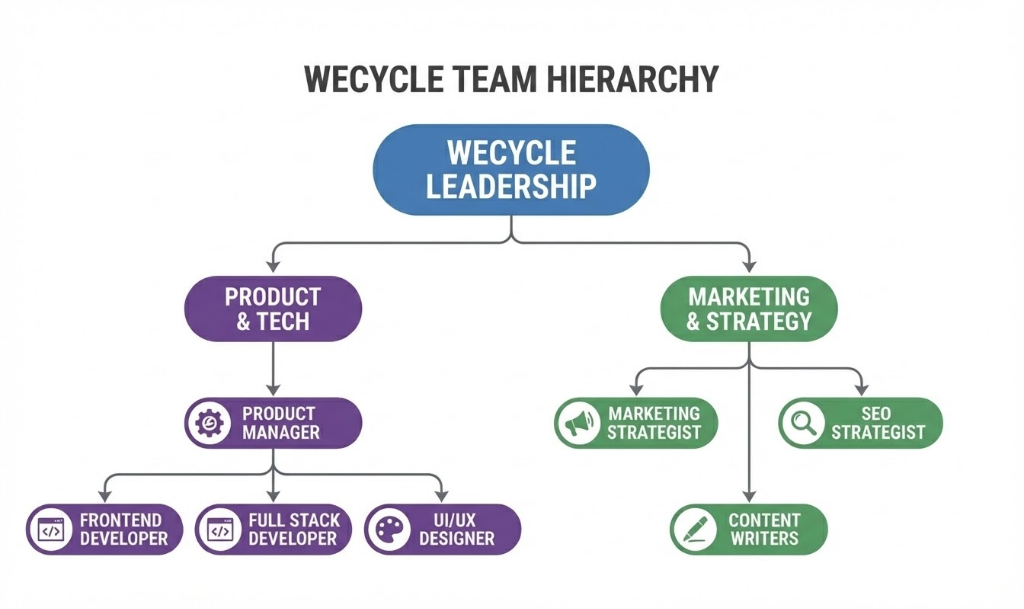
\includegraphics[width=0.85\textwidth]{figures/wecycle_org_structure.png}
    \caption{Tanbel Inc. (WeCycle) Organizational Structure}
    \label{fig:org-structure}
\end{figure}

\subsection{Interactions with Various Departments}
\par You can't code in a vacuum here. I talked to designers to make sure my pixels were perfect. I synced with the Operations team to understand *why* we were building a specific feature. And, of course, QA was always there to tell me when I broke something. It’s a constant loop of feedback and iteration. Communication happens everywhere—Slack, Standups, Jira comments. It keeps everyone on the same page.

\subsection{Collaboration with Team Leads}
\par Team leads here aren't just managers; they're mentors. They unblock you when you're stuck and review your code to make sure it's up to par. I reported directly to my industrial supervisor, but the whole team was fair game for questions. It was a mix of "here's how to do it" and "figure it out, then let's talk about it."

\subsection{Cross-Functional Coordination}
\par Building a feature involves everyone. We use Jira to track the madness and GitHub to manage the code. Slack is where the real work happens—quick questions, rapid decisions. It’s structured enough to be organized (Sprint Planning, Retrospectives) but loose enough to be fast.

\section{Products/Services}

\subsection{WeCycle Dashboard Application (WCAPP)}
\par The Dashboard is the engine. It handles everything. Leads? Yes. Payments? Yes. Crew management? Also yes. It’s the single point of failure and the single source of truth. It looks clean on the UI, but the logic underneath is massive.

Key features I worked with:

\begin{itemize}
    \item \textbf{Lead Management:} Tracking potential customers from "just looking" to "booked."
    \item \textbf{Client Management:} Keeping tabs on customer history and preferences.
    \item \textbf{Job Scheduling:} The calendar view is critical. It assigns jobs, tracks statuses, and sends reminders.
    \item \textbf{Hauler Management:} Managing the workforce—assignments, payouts, performance.
    \item \textbf{Invoicing:} Getting paid. Templates, tracking, automated billing.
    \item \textbf{Team Chat:} Built-in communication so we don't have to leave the app to talk.
\end{itemize}

\begin{figure}[H]
    \centering
    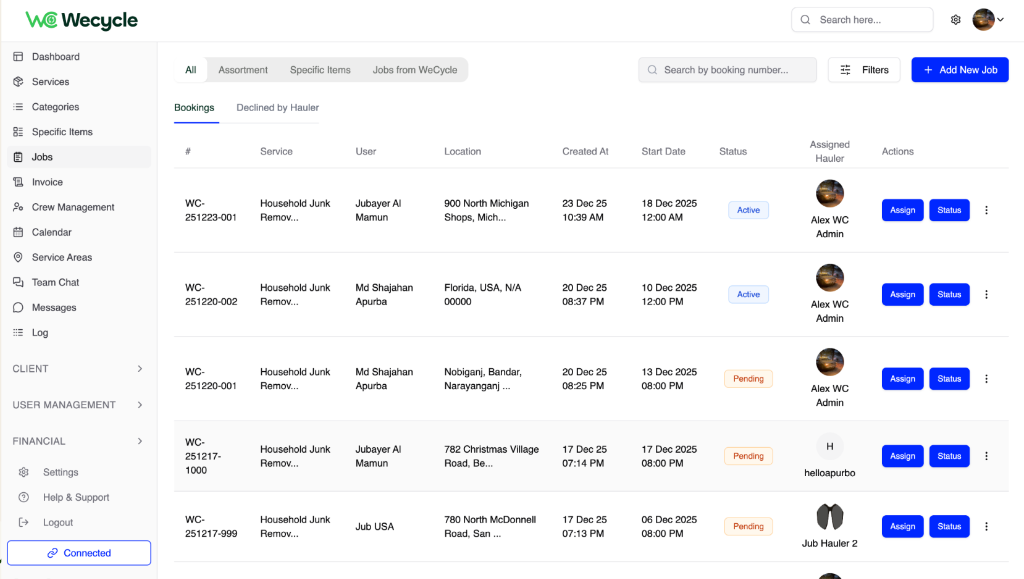
\includegraphics[width=0.95\textwidth]{figures/dashboard_jobs.png}
    \caption{WeCycle Dashboard - Job Scheduling and Management}
    \label{fig:dashboard-jobs}
\end{figure}

\begin{figure}[H]
    \centering
    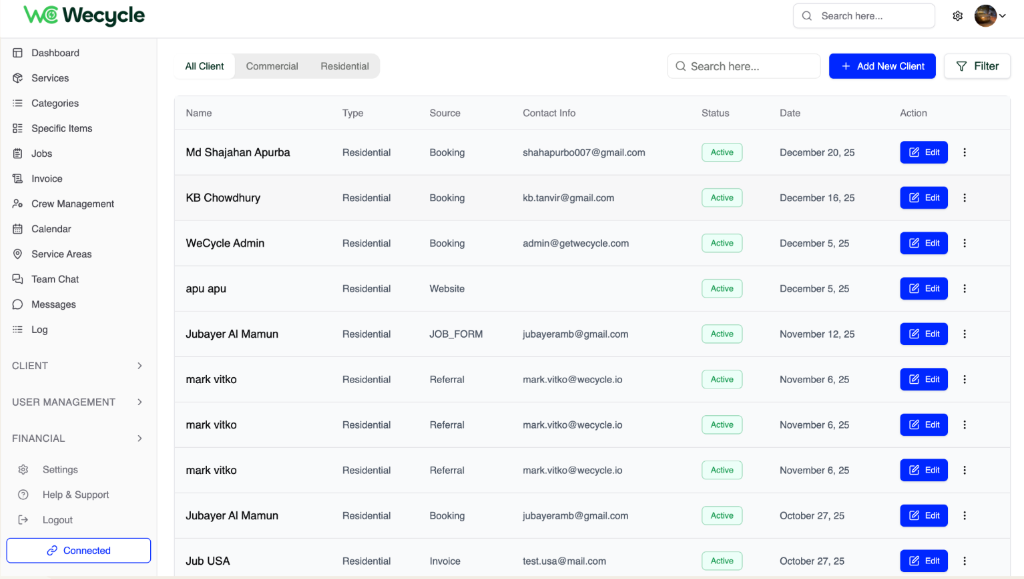
\includegraphics[width=0.95\textwidth]{figures/dashboard_clients.png}
    \caption{WeCycle Dashboard - Client Management}
    \label{fig:dashboard-clients}
\end{figure}

\begin{figure}[H]
    \centering
    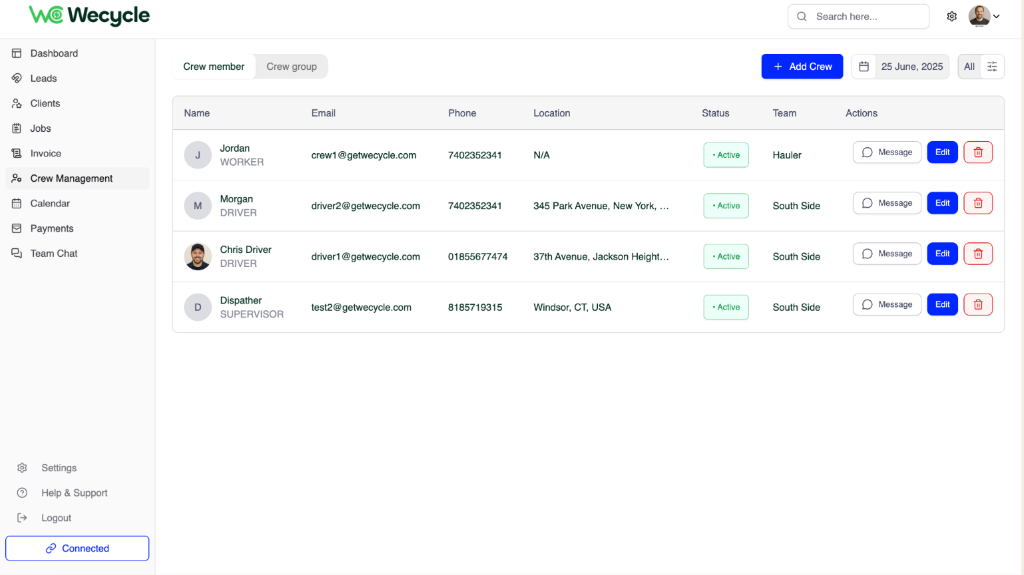
\includegraphics[width=0.95\textwidth]{figures/dashboard_crew.png}
    \caption{WeCycle Dashboard - Crew Management}
    \label{fig:dashboard-crew}
\end{figure}

\begin{figure}[H]
    \centering
    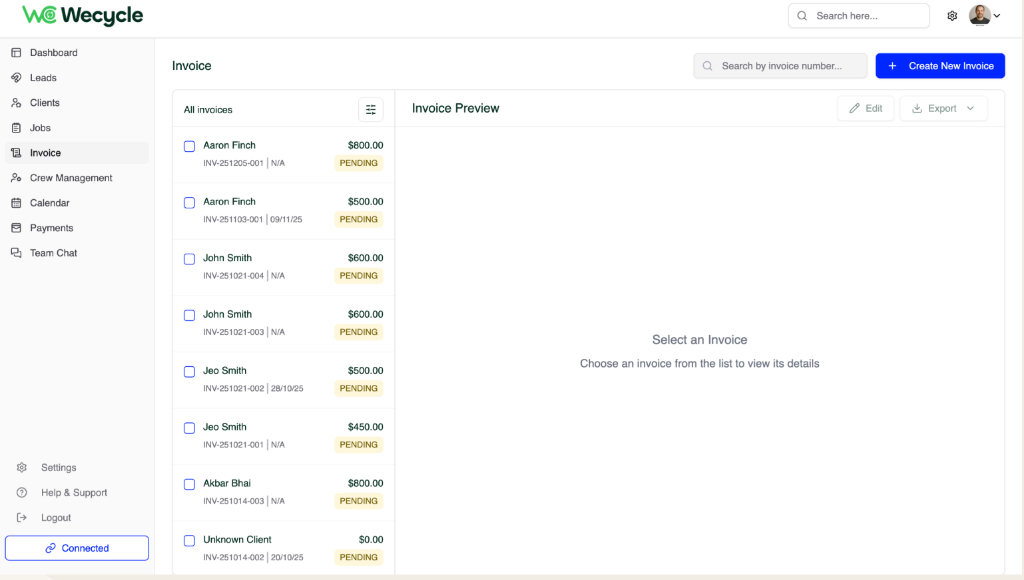
\includegraphics[width=0.95\textwidth]{figures/dashboard_invoice.png}
    \caption{WeCycle Dashboard - Invoice Management}
    \label{fig:dashboard-invoice}
\end{figure}

\begin{figure}[H]
    \centering
    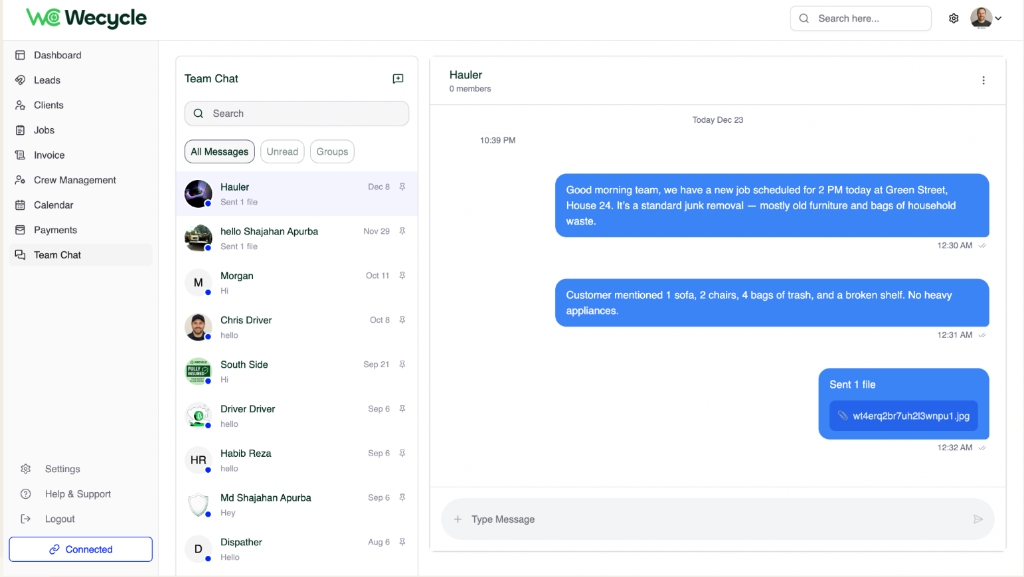
\includegraphics[width=0.95\textwidth]{figures/dashboard_teamchat.png}
    \caption{WeCycle Dashboard - Team Chat}
    \label{fig:dashboard-teamchat}
\end{figure}

\begin{figure}[H]
    \centering
    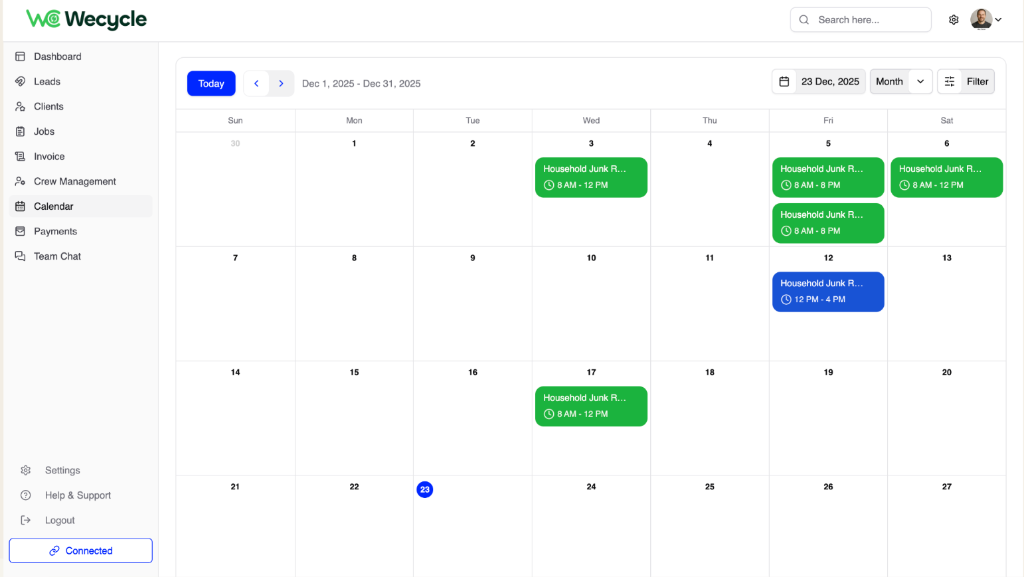
\includegraphics[width=0.95\textwidth]{figures/dashboard_calendar.png}
    \caption{WeCycle Dashboard - Calendar View}
    \label{fig:dashboard-calendar}
\end{figure}

\subsection{Technology Stack}
\begin{table}[H]
\centering
\caption{Technology Stack Configuration}
\begin{tabular}{|l|l|}
\hline
\textbf{Category} & \textbf{Technologies} \\
\hline
Frontend Framework & React.js, Next.js, Capacitor.js \\
\hline
Mobile Framework & React Native, Capacitor \\
\hline
Backend Environment & Node.js, Express.js \\
\hline
Database & MongoDB, PostgreSQL \\
\hline
Styling & Tailwind CSS, SCSS \\
\hline
Language & TypeScript, JavaScript \\
\hline
Build Tools & Nx, Vite \\
\hline
DevOps \& CI/CD & Docker, Nginx, GitHub Actions \\
\hline
Version Control & Git, GitHub \\
\hline
Project Management & Jira, Linear \\
\hline
\end{tabular}
\label{tab:tech-stack}
\end{table}

\section{Clients}
\par WeCycle is for everyone.
\begin{itemize}
    \item \textbf{Homeowners:} People cleaning out their garages or moving house.
    \item \textbf{Businesses:} Offices, retail stores, restaurants dealing with daily waste.
    \item \textbf{Property Managers:} Handling move-outs and large-scale cleanups.
    \item \textbf{Constructors:} Dealing with debris and renovation mess.
    \item \textbf{Events:} Because big parties make big messes.
\end{itemize}

\section{Direct Involvement of Resources During Training}
\begin{itemize}
    \item \textbf{Human Resources:}
    \begin{itemize}
        \item MD Tanvir Ahmed (My Supervisor): The go-to for code reviews and guidance.
        \item Senior Devs: For when I was completely stuck.
        \item UI/UX Designers: For the blueprints.
        \item Project Manager: For the deadlines.
    \end{itemize}
    \item \textbf{Technical Resources:}
    \begin{itemize}
        \item My Laptop (obvious, but essential).
        \item GitHub Access (the keys to the castle).
        \item Jira (the taskmaster).
        \item Staging Environment (the playground).
        \item Chrome DevTools (the microscope).
    \end{itemize}
\end{itemize}

\section{Constructive Feedback About the Training Program}
\par Honesty time.
\begin{itemize}
    \item \textbf{The Good Stuff:}
    \begin{itemize}
        \item Real work. No fetching coffee. I wrote production code.
        \item The stack is modern. React and Next.js are what everyone wants right now.
        \item flexibility. Remote work is a game-changer.
    \end{itemize}
    \item \textbf{The "Could Be Better" Stuff:}
    \begin{itemize}
        \item Documentation was... sparse. A better "Getting Started" guide would save days of confusion.
        \item More pair programming would speed up the learning curve.
    \end{itemize}
    \item \textbf{Advice for the Next Intern:}
    \begin{itemize}
        \item Learn React before you start. Seriously.
        \item Ask questions. Sitting in silence when you're stuck is a waste of time.
        \item Map out the codebase early. It helps.
    \end{itemize}
\end{itemize}

\section{Conclusion}
\par Tanbel Inc. is flat. No layers of bureaucracy slowing you down. That's why it moves fast. The team cares about innovation, but also about customers and the planet—it's not just marketing talk. The development practices are modern: React, Next.js, clean code reviews. It's a real place to learn Full-Stack development. Beyond just building features, the company is doing something useful—making waste disposal smarter and pushing recycling over dumping. For a first real job, it checks every box: tech that matters, a culture that values learning, and work that actually makes a difference.    